\documentclass{standalone}
\usepackage{graphicx}	
\usepackage{amssymb, amsmath}
\usepackage{color}

\usepackage{tikz}
\usetikzlibrary{intersections, backgrounds, patterns, patterns.meta}
\usepackage{pgfmath}

\definecolor{light}{RGB}{220, 188, 188}
\definecolor{mid}{RGB}{185, 124, 124}
\definecolor{dark}{RGB}{143, 39, 39}
\definecolor{highlight}{RGB}{180, 31, 180}
\definecolor{gray10}{gray}{0.1}
\definecolor{gray20}{gray}{0.2}
\definecolor{gray30}{gray}{0.3}
\definecolor{gray40}{gray}{0.4}
\definecolor{gray60}{gray}{0.6}
\definecolor{gray70}{gray}{0.7}
\definecolor{gray80}{gray}{0.8}
\definecolor{gray90}{gray}{0.9}
\definecolor{gray95}{gray}{0.95}

\begin{document}

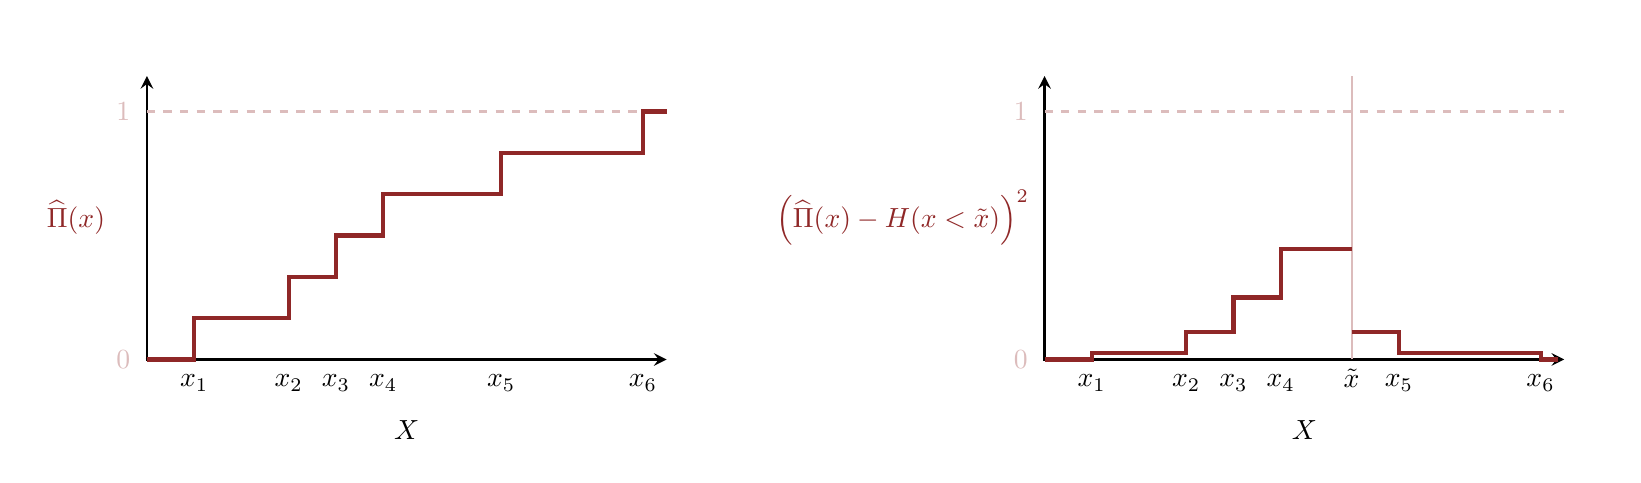
\begin{tikzpicture}[scale=0.3, thick]

\begin{scope}[shift={(0, 0)}]
  \draw[white] (-16, -4) rectangle (13, 14);

  \node[dark] at (-14, 6) { $\widehat{\Pi}(x)$ };
  
  \draw [->, >=stealth, line width=1] (-11, 0) -- (-11, 12);

  \draw [->, >=stealth, line width=1] (-11.05, 0) -- (11, 0);
  \node at (0, -3) { $X$ };
  
  \draw[light, dashed] (-11, 10.5) -- (11, 10.5);
  \node[light] at (-12, 10.5) { $1$ };
  \node[light] at (-12, 0) { $0$ };
  
  \draw[dark, line width=1.5] (-11, 0) -- 
                              (-9, 0) -- (-9, 1.75) -- 
                              (-5, 1.75) -- (-5, 3.5) -- 
                              (-3, 3.5) -- (-3, 5.25) -- 
                              (-1, 5.25) -- (-1, 7) --
                              (4, 7) -- (4, 8.75) --
                              (10, 8.75) -- (10, 10.5) --
                              (11, 10.5);
  
  \node at (-9, -1) { $x_{1}$ };
  \node at (-5, -1) { $x_{2}$ };
  \node at (-3, -1) { $x_{3}$ };
  \node at (-1, -1) { $x_{4}$ }; 
  \node at (+4, -1) { $x_{5}$ };   
  \node at (+10, -1) { $x_{6}$ };
  
\end{scope}

\begin{scope}[shift={(38, 0)}]
  \draw[white] (-23, -4) rectangle (13, 14);

  \node[dark] at (-17, 6) { $\Big( \widehat{\Pi}(x) - H(x < \tilde{x}) \Big)^{2}$ };
  
  \draw [->, >=stealth, line width=1] (-11, 0) -- (-11, 12);

  \draw [->, >=stealth, line width=1] (-11.05, 0) -- (11, 0);
  \node at (0, -3) { $X$ };
  
  \draw[light, dashed] (-11, 10.5) -- (11, 10.5);
  \node[light] at (-12, 10.5) { $1$ };
  \node[light] at (-12, 0) { $0$ };
  
  \draw[light] (2, 0) -- (2, 12);
  \node at (+2, -0.775) { $\tilde{x}$ };
  
  \draw[dark, line width=1.5] (-11, 0) -- 
                              (-9, 0) -- (-9, {1 * 1 * 10.5 / 36}) -- 
                              (-5, {1 * 1 * 10.5 / 36}) -- (-5, {2 * 2 * 10.5 / 36}) -- 
                              (-3, {2 * 2 * 10.5 / 36}) -- (-3, {3 * 3 * 10.5 / 36}) -- 
                              (-1, {3 * 3 * 10.5 / 36}) -- (-1, {4 * 4 * 10.5 / 36}) --
                              (2,  {4 * 4 * 10.5 / 36});

  \draw[dark, line width=1.5] (2, {(6 - 4) * (6 - 4) * 10.5 / 36}) --
                              (4, {(6 - 4) * (6 - 4) * 10.5 / 36}) -- (4, {(6 - 5) * (6 - 5) * 10.5 / 36}) --
                              (10, {(6 - 5) * (6 - 5) * 10.5 / 36}) -- (10, {(6 - 6) * (6 - 6) * 10.5 / 36}) --
                              (10.75, {(6 - 6) * (6 - 6) * 10.5 / 36});  
  
  \node at (-9, -1) { $x_{1}$ };
  \node at (-5, -1) { $x_{2}$ };
  \node at (-3, -1) { $x_{3}$ };
  \node at (-1, -1) { $x_{4}$ }; 
  \node at (+4, -1) { $x_{5}$ };   
  \node at (+10, -1) { $x_{6}$ };
  
\end{scope}
  
\end{tikzpicture}

\end{document}  